\chapter{Experimentación}\label{ch:Experimentación}

Esta sección tiene como objetivo mostrar el correcto funcionamiento las funciones documentadas en la Sección \ref{ch:Impl}. Para ello las aplicaremos sobre conjuntos de datos correspondientes a casos de aplicación reales, así como a conjuntos artificiales.

Cabe destacar que los parámetros dados como argumento a las funciones son los especificados por defecto en la Sección \ref{ch:Impl} a no ser que se especifique lo contrario, es decir, no se han optimizado para los datos concretos a los que se aplican en cada ocasión. La optimización de parámetros queda a cargo del usuario, que deberá realizar un estudio sobre los mismos para adaptarlos al problema concreto que intenta resolver.

\section{Conjuntos de datos considerados} \label{datasets}

Tal y como ya se ha mencionado, tomaremos conjuntos de datos reales y artificiales para poner a prueba los 5 métodos implementados. Teniendo en cuenta dicha distinción, a continuación se detallan los pormenores de cada uno de ellos.

\subsection{Conjuntos de datos reales}

Consideraremos 4 conjuntos de datos correspondientes a casos reales de aplicación de técnicas de \acf{AA}:

\begin{itemize}
	
	\item \textbf{Conjunto de datos \textit{Iris}}: el conjunto de datos Iris (\textit{Iris dataset}) es uno de los más empleados en \acs{AA}. Famoso por ser objeto del primer intento de aplicación de métodos de clustering por el biólogo Ronald Fisher en 1936, quien intentaba obtener un método para clasificar flores de la especie Iris en sus tres subespecies: \textit{iris setosa}, \textit{iris virginica} e \textit{iris versicolor}. Compuesto por un total de 150 muestras de 3 clases distintas, caracterizadas cada una por 4 atributos en el dominio de los números reales positivos, a saber: altura del sépalo, anchura del sépalo, altura del pétalo y anchura del pétalo.
	
	\item \textbf{Conjunto de datos \textit{Wine}}: el conjunto de datos Wine (\textit{Wine dataset}) recoge 178 muestras de 3 clases de vinos distintas, caracterizadas cada una por 13 atributos en el dominio de los números reales positivos. Algunos de estos atributos son: contenido de alcohol, contenido de ácido málico, contenido de magnesio, etc.
	
	\item \textbf{Conjunto de datos \textit{Breast Cancer}}: el conjunto de datos Breast Cancer (\textit{Breast Cancer dataset}) recoge 569 asociadas cada una a una paciente que padecía o no de cáncer de mama (2 clases), cada muestra viene caracterizada por 30 atributos en el dominio de los números reales positivos. Algunos de los atributos son: edad de la paciente, tamaño del tumor, mama afectada, etc.
	
	\item \textbf{Conjunto de datos \textit{Glass}}: el conjunto de datos Glass (\textit{Glass dataset}) recoge 214 muestras de 6 clases de cristal distintas, caracterizadas cada una por 10 atributos en multitud de dominios. Algunos de estos atributos son: indice reactivo, contenido en magnesio, contenido en aluminio, finalidad de uso, etc.
	
\end{itemize}

\subsection{Conjuntos de datos artificiales}

En el caso de los conjuntos de datos artificiales el objetivo es generar clusters con una geometría concreta, para ello sólo son necesarios dos atributos ($x$ e $y$) y un número de muestras arbitrario.

La Figura \ref{fig:figure22} muestran los 4 conjuntos de datos generados de manera artificial. Por simplicidad nos referiremos a cada uno de ellos por su identificador en ingles, que aparece en la anotación bajo cada imagen.

\begin{figure}[bth]
	\myfloatalign
	\subfloat[\textit{Rand Dataset}]
	{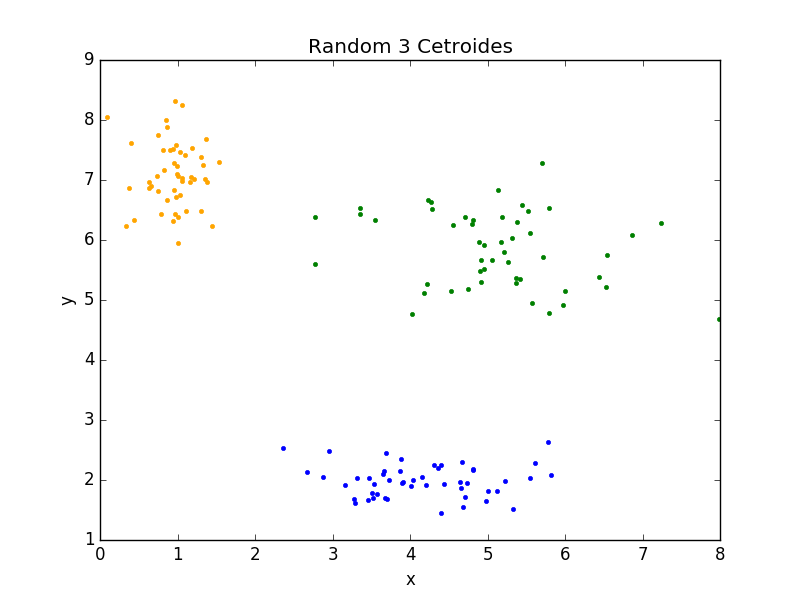
\includegraphics[width=.4\linewidth]{imagenes/c6/ArtifSets/RandSet}}
	\subfloat[\textit{Spirals Dataset}]
	{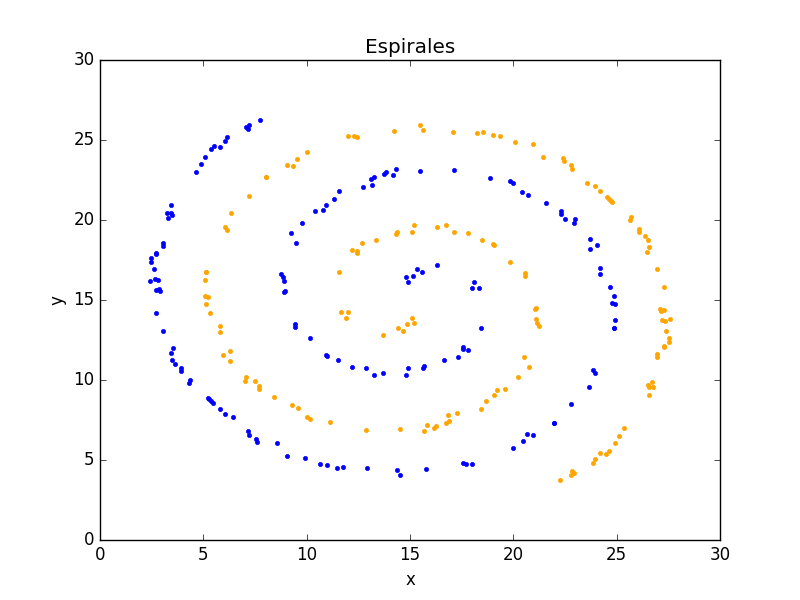
\includegraphics[width=.4\linewidth]{imagenes/c6/ArtifSets/SpiralSet}}\\
	\subfloat[\textit{Circles Dataset}]
	{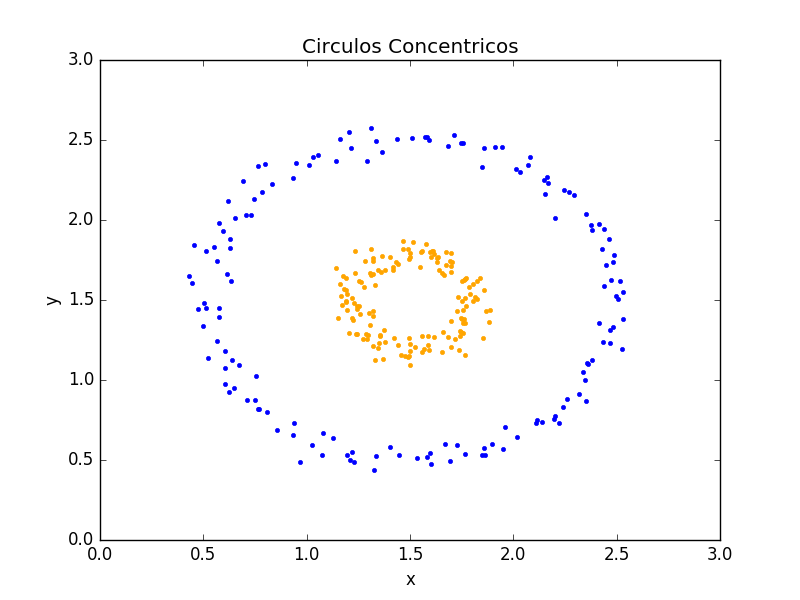
\includegraphics[width=.4\linewidth]{imagenes/c6/ArtifSets/Circles}}
	\subfloat[\textit{Moons Dataset}]
	{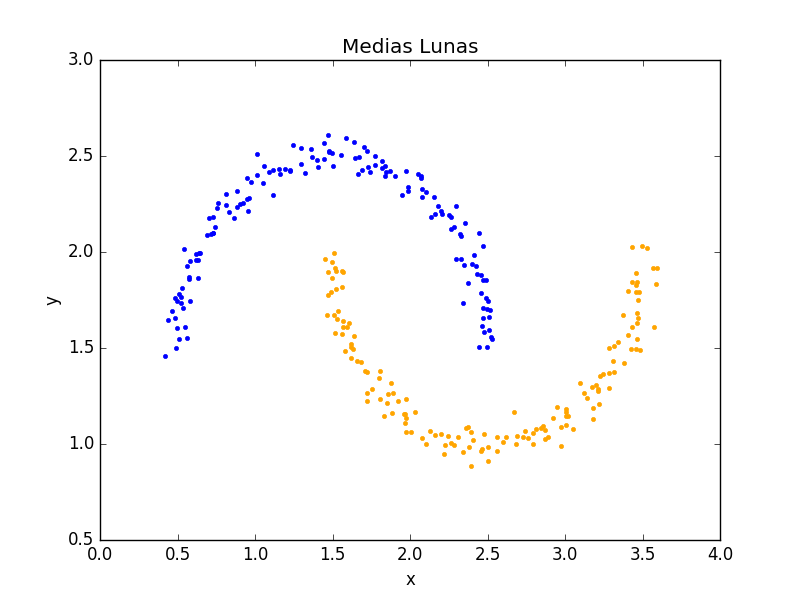
\includegraphics[width=.4\linewidth]{imagenes/c6/ArtifSets/MoonsSet}}
	\caption{Conjuntos de datos artificiales.}\label{fig:figure22}
\end{figure}

\section{Medida del error}

Tomamos la medida del error que Wagstaff et al. (2001) \cite{Wagstaff:2001b}, los autores de COP-K-medias, proponen en su trabajo para evaluar los resultados.

Dado que en la experimentación disponemos de las etiquetas verdaderas asociadas a cada uno de los conjuntos de datos, podemos hacer uso de las mismas en el post-procesado para evaluar los resultados que proporciona cada método.

Para calcular la exactitud de las predicciones resultado de cada método emplearemos \textit{Rand Index} \cite{Rand:1971}, que calcula el grado de similitud entre dos particiones dadas $P_1$ y $P_2$ del mismo conjunto de datos $X$.

Interpretamos cada partición como una colección de $n (n-1) / 2$ decisiones de emparejamiento, donde $n$ es el número de instancias en $X$. Para cada par de instancias $x_i$ y $x_j$ en $X$, $P_i$ las asigna al mismo cluster o a clusters diferentes. Tomamos $a$ como el número de emparejamientos donde $x_i$ está en el mismo cluster que $x_j$ en $P_1$ y $P_2$, y tomamos $b$ como el suceso contrario. Entonces, el grado de similitud entre $P_1$ y $P_2$ se calcula como:

\begin{equation}
Rand(P_1, P_2) = \frac{a + b}{n (n-1) / 2}
\label{eqn70}
\end{equation}

Esta será la medida del error que emplearemos en todos los experimentos.

\section{Generación de las restricciones}

Para generar las restricciones haremos uso de la función propuesta para ello en la Sección \ref{genConst}. La cantidad de restricciones viene definida como un porcentaje aplicado sobre el cardinal de conjunto de datos. Dicho porcentaje se especificará en la sección correspondiente al análisis de cada algoritmo. No obstante, podemos obtener una representación gráfica de las restricciones haciendo uso de las funcionalidades de la biblioteca Matplotlib, la Figura \ref{fig:figure23} muestra las restricciones generadas sobre los conjuntos de datos \textit{Rand Dataset} e \textit{Rand Dataset}, especificando que el número de restricciones debe ser un $30\%$ del total de los datos disponibles en cada caso.



\begin{figure}[bth]
	\myfloatalign
	\subfloat[\textit{Iris Dataset}]
	{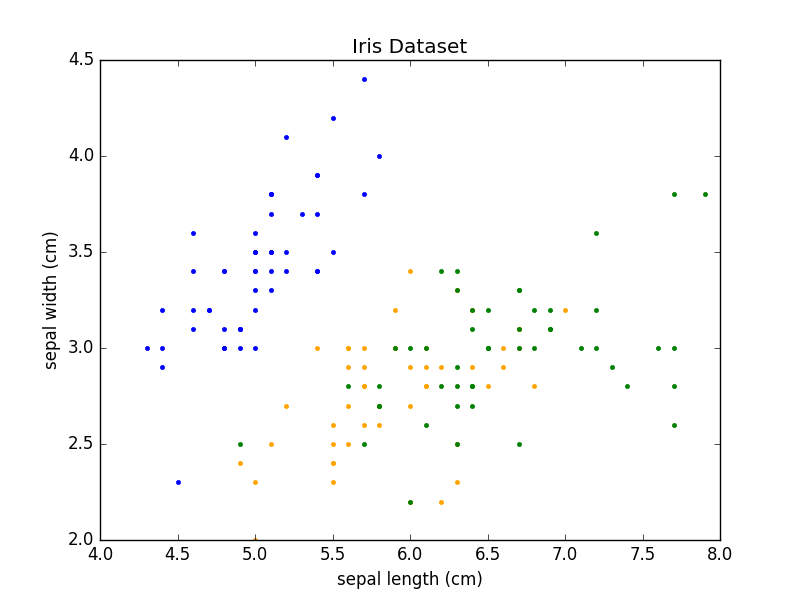
\includegraphics[width=.3\linewidth]{imagenes/c6/IrisSet}}
	\subfloat[\textit{Restricciones \acs{ML}}]
	{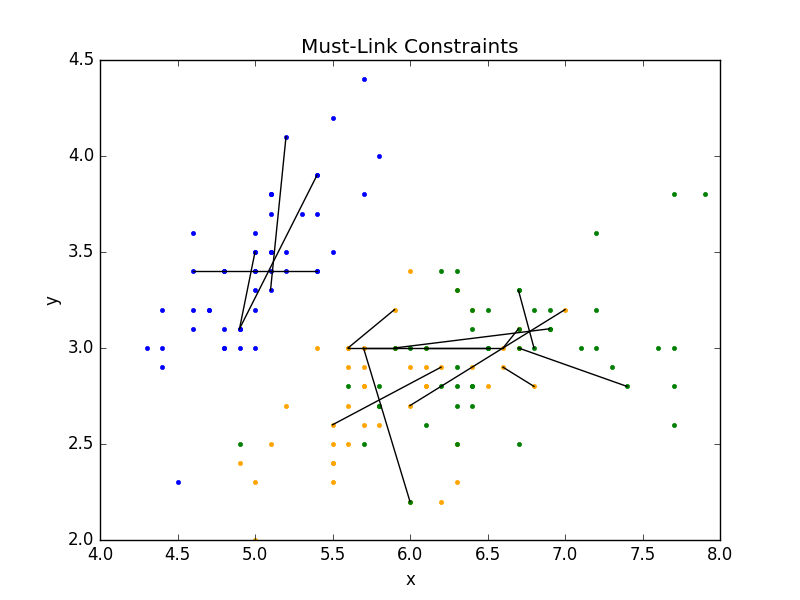
\includegraphics[width=.3\linewidth]{imagenes/c6/Restr/IrisML}}
	\subfloat[\textit{Restricciones \acs{CL}}]
	{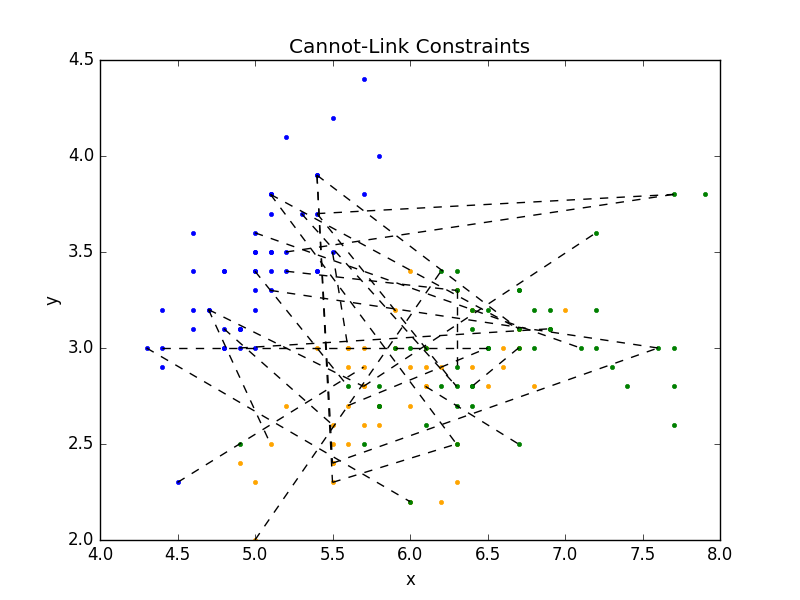
\includegraphics[width=.3\linewidth]{imagenes/c6/Restr/IrisCL}}\\
	\subfloat[\textit{Rand Dataset}]
	{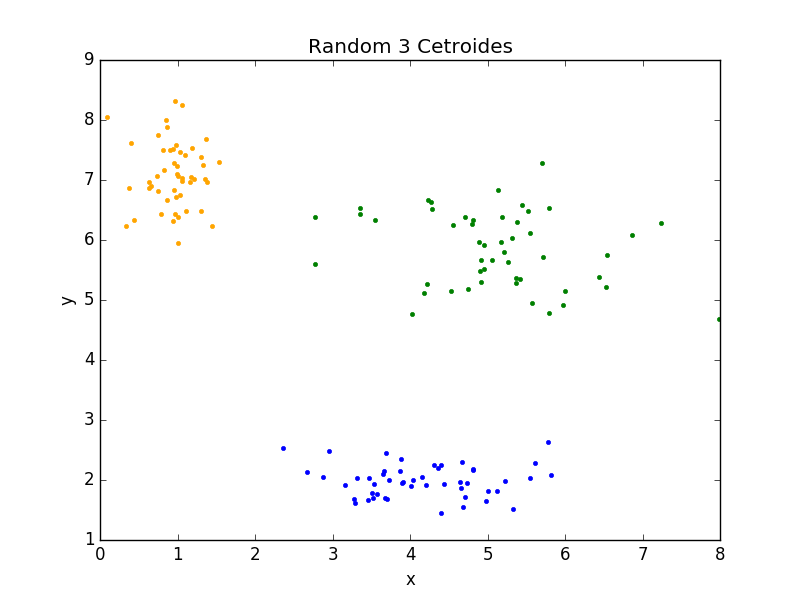
\includegraphics[width=.3\linewidth]{imagenes/c6/ArtifSets/RandSet}}
	\subfloat[\textit{Restricciones \acs{ML}}]
	{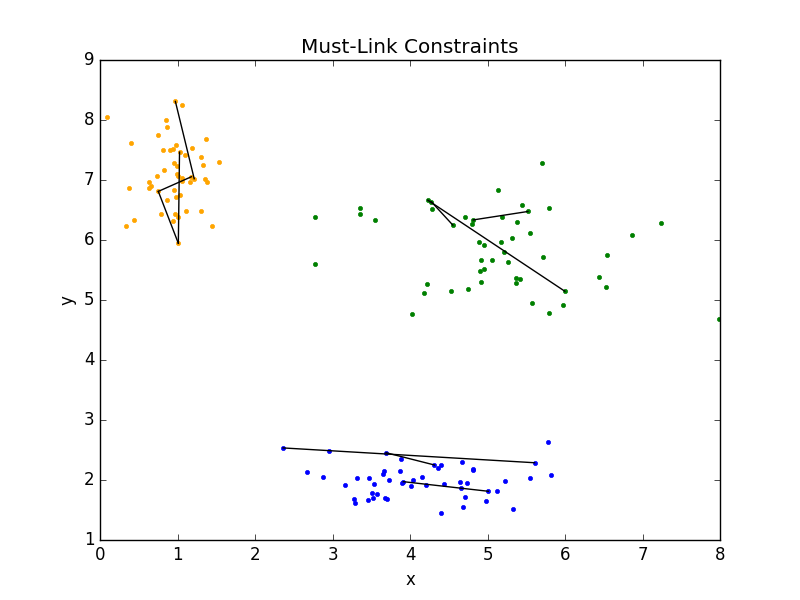
\includegraphics[width=.3\linewidth]{imagenes/c6/Restr/RandML}}
	\subfloat[\textit{Restricciones \acs{CL}}]
	{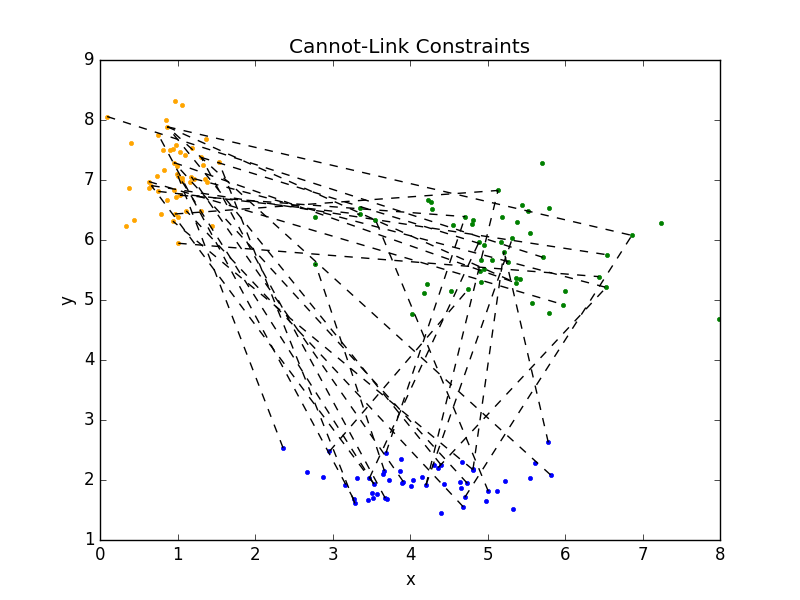
\includegraphics[width=.3\linewidth]{imagenes/c6/Restr/RandCL}}\\
	\caption{Visualización de las restricciones.}\label{fig:figure23}
\end{figure} 

\section{Resultados de COP-K-Medias}

A continuación se muestran los resultados obtenidos al aplicar el algoritmo COP-K-Medias (Sección \ref{copkm}) a los conjuntos de datos presentados en la Sección \ref{datasets}.









